% Plantilla latex para protocolo de tesis de posgrado en la Facultad de Ingeniería, Universidad Autónoma de Querétaro.
%
% @author {Edgar Lara Arellano}
% @email {elara28@alumnos.uaq.mx}
% @year 2024
% @version 1.0
% @license CC-BY-NC
%
% Se agradecen sus comentarios, contribuciones,  reporte de bugs y la difusión de esta plantilla


% Logos tomados de: https://ingenieria.uaq.mx/index.php/descargas
% Elementos complementarios tomados de: https://www.uaq.mx/f_ingenieria/images/Assets_web_ing/PAQUETE_GRAFICO_FI_PARA_DESCARGA/Manual_identidad_oficil_fi/MANUAL-OFICIAL-FI-2019.pdf

%Plantilla basada en los requerimientos planteados en [Guía para la escritura de Tésis, FI, UAQ](https://dip.uaq.mx/docs/posgrado/Guia-tesis-CNyE.pdf)



\documentclass[12pt, letterpaper, spanish, twoside]{article}
\AddToHook{cmd/section/before}{\newpage}
\usepackage{./common/UAQ}

\graphicspath{{./figures/}}


\begin{document}


%\documentclass[12pt]{article}


% Margins
%\usepackage[a4paper, left=3cm, right=3cm, top=3cm, bottom=3cm]{geometry}



\backgroundsetup{
	scale = 1,
	angle = 0,
	opacity = 1,
	contents = {
		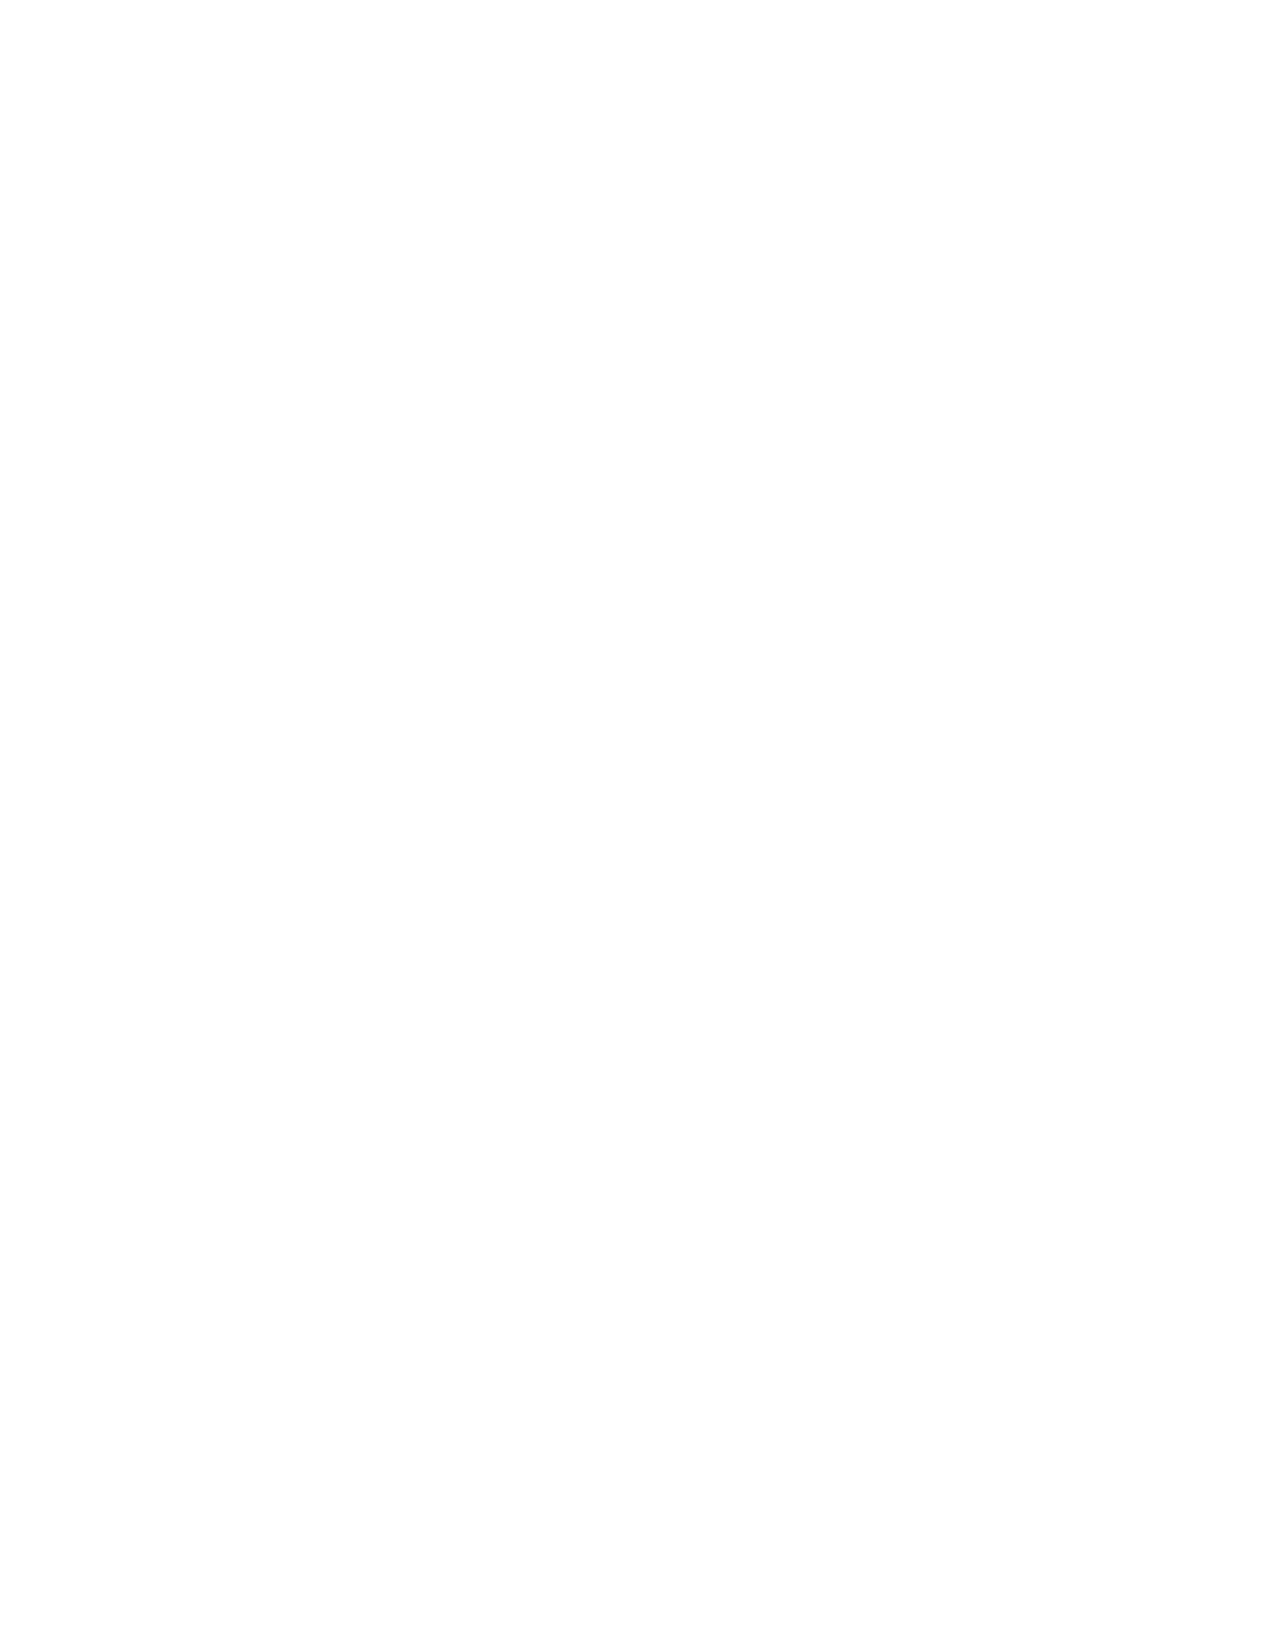
\includegraphics[width=\paperwidth]{figures/externalCoverBackground.pdf}
	}
}

%\AtBeginShipoutFirst{\AtBeginShipoutDiscard}
% No page numbers
\pagestyle{empty}
    \begin{minipage}[H][\textheight][c]{0.15\textwidth}
        \begin{tcolorbox}[colframe=black, colback=white, rounded corners, boxrule=0.5mm, width=\linewidth, height=\textheight, valign=center]
            \begin{center}
                \rotatebox{90}{\large \textbf{Autor}} \\
                \vspace{2cm}
                \rotatebox{90}{\large \textbf{Nombre de la tesis}} \\
                \vspace{2cm}
                \rotatebox{90}{\large \textbf{Año}} \\
            \end{center}
        \end{tcolorbox}
    \end{minipage}
    \hfill
    \begin{minipage}[H][\textheight][c]{0.8\textwidth}
    
        \begin{tcolorbox}[colframe=black, colback=white, rounded corners, boxrule=0.5mm, width=\linewidth, height=\textheight, valign=center]
            \begin{minipage}[t][3cm][c]{0.2\textwidth}

            \vspace{2cm}
                
\includegraphics[width=\linewidth]{figures/logo_UAQ.png} % Replace with the logo of the university
            \end{minipage}
            \hfill
            \begin{minipage}[t][3cm][c]{0.7\textwidth}
                \begin{center}
                \vspace{2cm}
                    {\Large \textbf{Universidad Autónoma de Querétaro}} \\
                    \vspace{0.2cm}
                    {\large \textbf{Facultad de \underline{\hspace{3cm}}}} \\
                \end{center}
            \end{minipage}
            
            \vspace{2cm}
            
            \begin{center}
                {\Large \textbf{Título del tema de tesis registrado}} \\
                \vspace{1cm}
                {\Large \textbf{Tesis}} \\
                \vspace{0.5cm}
                {\large Que como parte de los requisitos para obtener el Grado de} \\
                \vspace{0.5cm}
                {\large \textbf{Maestro/Doctor en}} \\
                \vspace{1cm}
                \hrule height 0.4mm width 9cm
                \vspace{1cm}
                {\large Presenta} \\
                \vspace{0.5cm}
                {\Large \textbf{Nombre del aspirante}} \\
            \end{center}
            
            \vspace{2cm}
            
            \begin{flushleft}
                \textbf{Dirigido por:} \\
                \textbf{Nombre completo del Director del Tesis} \\
                \vspace{0.5cm}
                \textbf{Co-Director:} \\
                \textbf{Nombre completo del Co-Director de tesis (en su caso)} \\
            \end{flushleft}
            
            \vfill
            
            \begin{flushright}
                \textbf{Querétaro, Qro. a \underline{\hspace{3cm}}} \\
            \end{flushright}
            
            \vspace{1cm}
        \end{tcolorbox}
    \end{minipage}




\backgroundsetup{
	scale = 1,
	angle = 0,
	opacity = 1,
	contents = {
		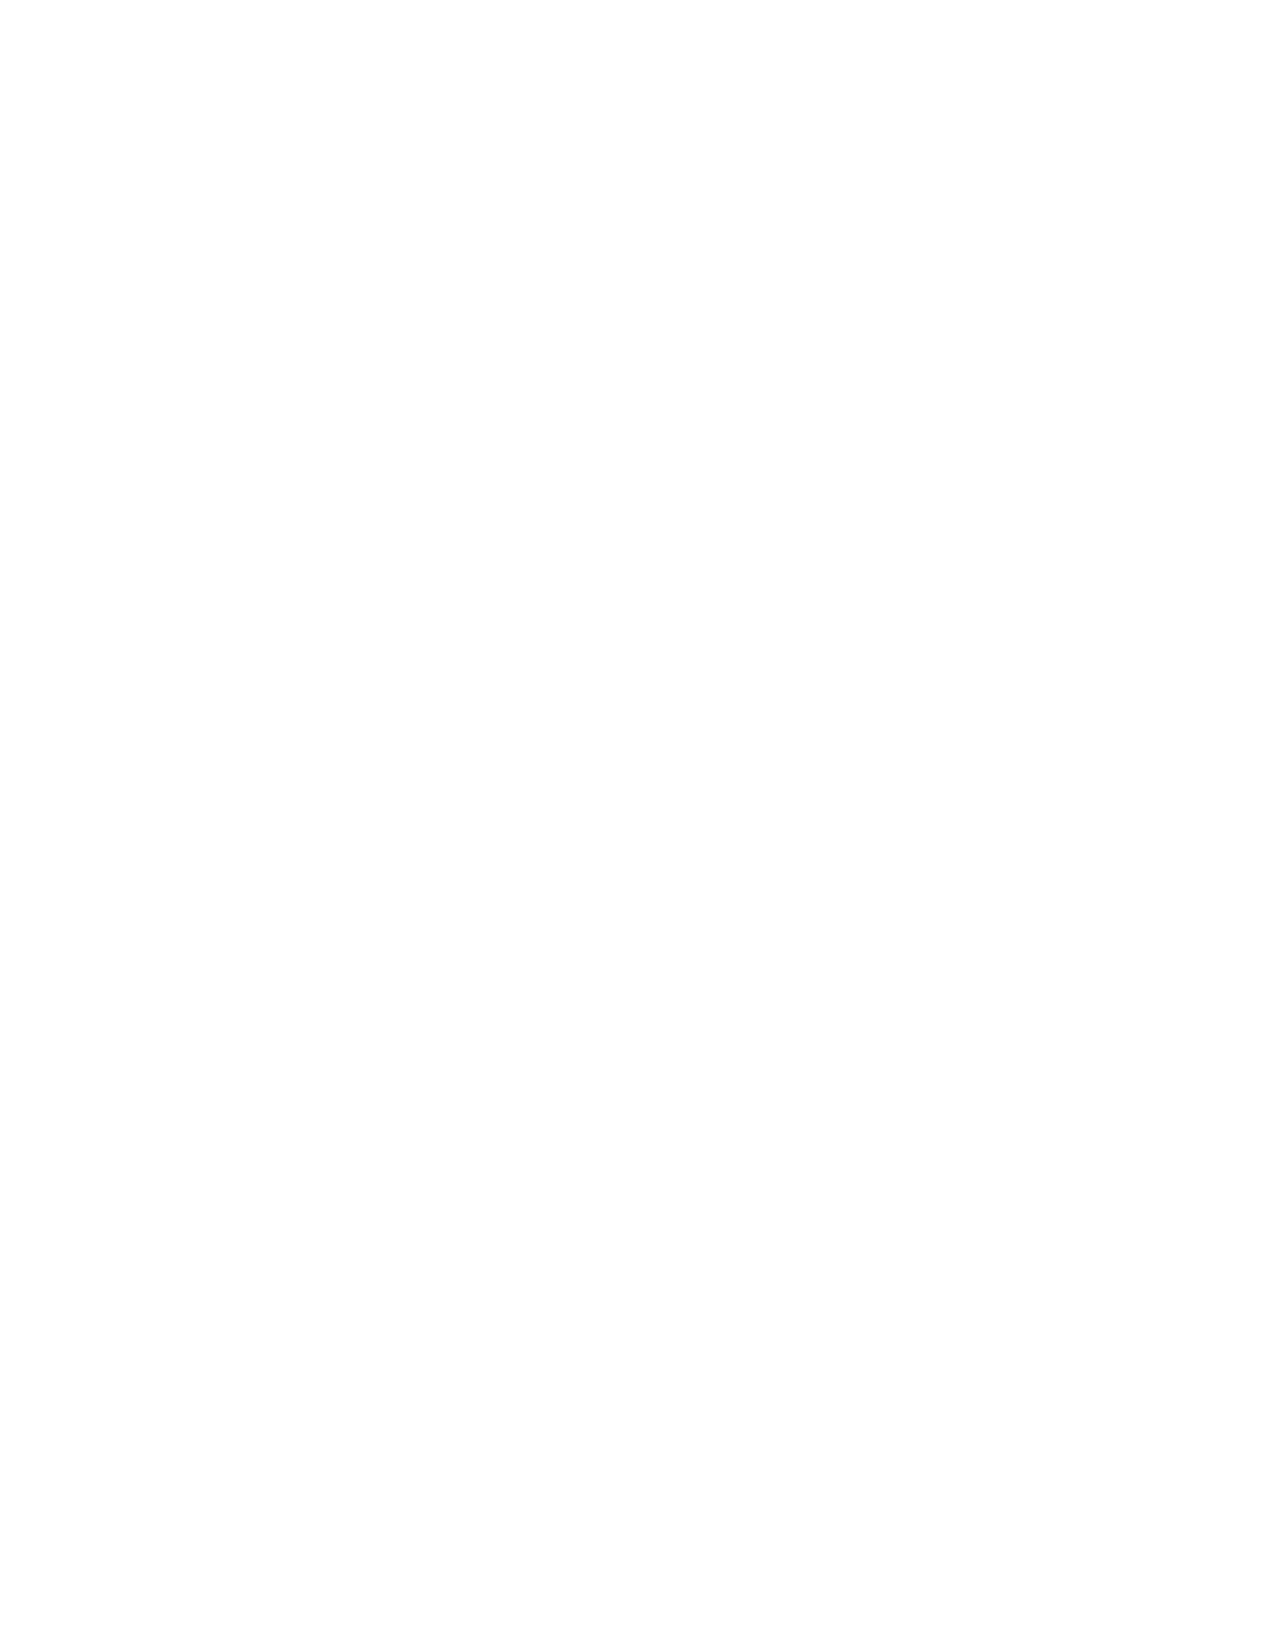
\includegraphics[width=\paperwidth]{figures/externalCoverBackground.pdf}
	}
}


\begin{minipage}[t][0cm][c]{0.2\textwidth}
                
\includegraphics[width=\linewidth]{figures/logo_UAQ.png} % Replace with the logo of the university
            \end{minipage}
            \hfill
            \begin{minipage}[t][0cm][c]{0.7\textwidth}
                \begin{raggedright}
                    {\Large \textbf{Universidad Autónoma de Querétaro}} \\
                    \vspace{0.2cm}
                    {\large \textbf{Facultad de \underline{\hspace{3cm}}}} \\
                    \vspace{0.2cm}
                    {\large \textbf{Maestría/Doctorado \underline{\hspace{3cm}}}} \\
                \end{raggedright}
            \end{minipage}

            \vspace{2cm}
            
            \begin{center}
                {\Large \textbf{Título del tema de tesis registrado}} \\
                \vspace{.8cm}
                {\Large \textbf{Tesis}} \\
                \vspace{0.5cm}
                {\large Que como parte de los requisitos para obtener el Grado de} \\
                \vspace{0.5cm}
                {\large \textbf{Maestro/Doctor en \underline{\hspace{3cm}}}}
                
                \vspace{1cm}
                {\large Presenta} \\
                \vspace{0.5cm}
                {\large \underline{\textbf{Nombre del aspirante}}} \\

                \vspace{1cm}
                {\large Dirigido por} \\
                \vspace{0.5cm}
                {\large \underline{\textbf{Nombre completo del Director de tesis}}} \\
            \end{center}
\vspace{1cm}
    \begin{flushleft}
        Nombre del Sinodal\\
        Presidente\\
        \vspace{.2cm}
        Nombre del Sinodal\\
        Secretario\\
        \vspace{.2cm}
        Nombre del Sinodal\\
        Vocal\\
        \vspace{.2cm}
        Nombre del Sinodal\\
        Suplente\\
        \vspace{.2cm}
        Nombre del Sinodal\\
        Suplente
        \vspace{.2cm}
    \end{flushleft}

\begin{center}
    Centro Universitario, Querétaro, Qro. México\\
Fecha de aprobación por el Consejo Universitario (mes y año)
\end{center}

\newpage

\backgroundsetup{
	scale = 1,
	angle = 0,
	opacity = 1,
	contents = {
		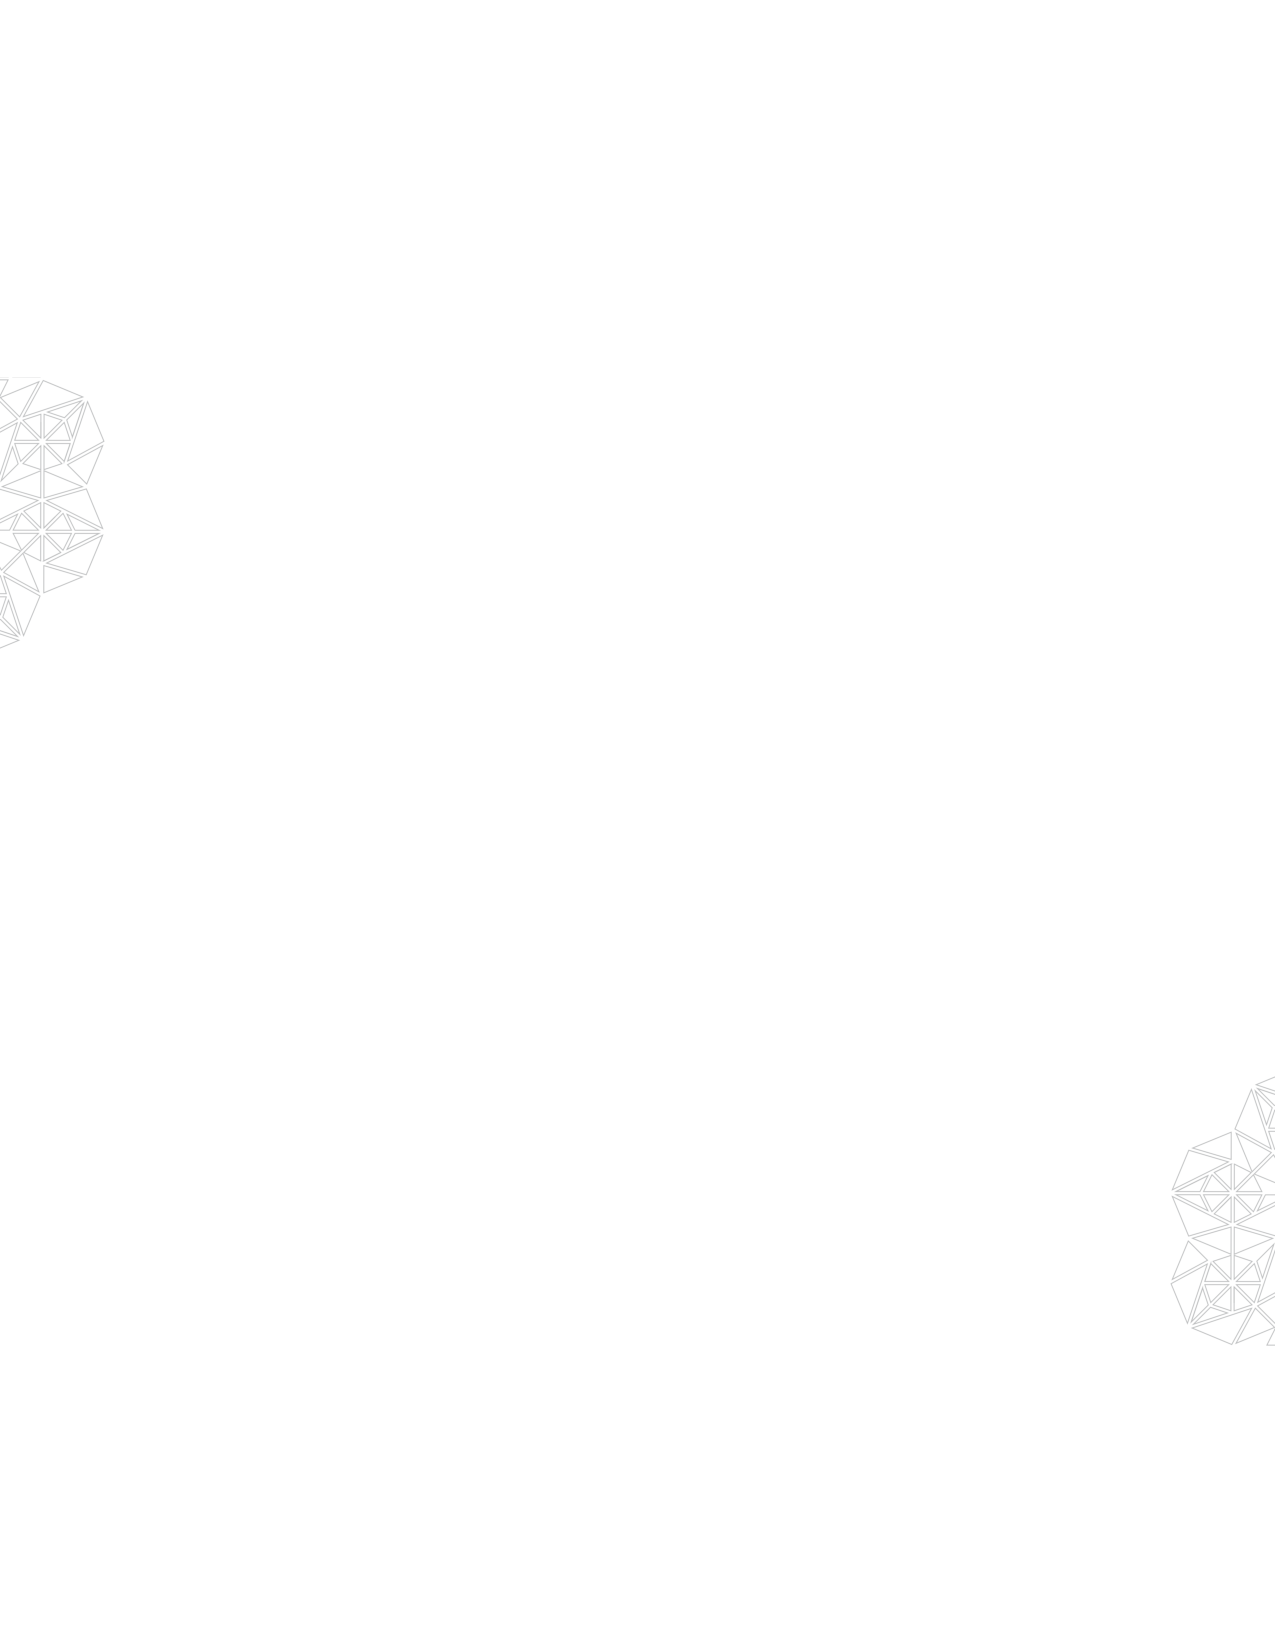
\includegraphics[width=\paperwidth]{figures/CoverBackground.pdf}
	}
}


\pagestyle{empty}

\begin{flushright}
    \vspace*{5cm}
    Dedicatorias: Este apartado es opcional.
\end{flushright}

\newpage
\pagestyle{empty}

\begin{center}
    {\Large{Agradecimientos}}
\end{center}


Serán personales, académicos y/o institucionales.
En el caso de los estudiantes que hayan recibido beca o financiamiento
para su trabajo final, deberán agradecer a la institución que le otorgó
la beca y/o el financiamiento.

\newpage
{\large \color{GrisUAQ} \textbf{Abreviaturas y siglas}}\\
Es opcional el listado de abreviaturas y/o siglas.

\newpage
{\large \color{GrisUAQ} \textbf{Resumen}}\\
Deberá ser escrito a renglón seguido y debe presentar de forma clara y concreta el planteamiento del problema, objetivos, metodología, y principales resultados. Tendrá una extensión máxima de 350 palabras. En la parte inferior incluir de 3 a 5 palabras claves para la descripción del contenido del documento.

\vspace{2cm}
{\large \color{GrisUAQ} \textbf{Abstract}}\\
Es la traducción del resumen en español, al igual que este deberá incluir palabras clave (keywords). Este resumen será revisado en corrección y estilo, por el comité de tesis.
\newpage
\backgroundsetup{
	scale = 1,
	angle = 0,
	opacity = 1,
	contents = {
		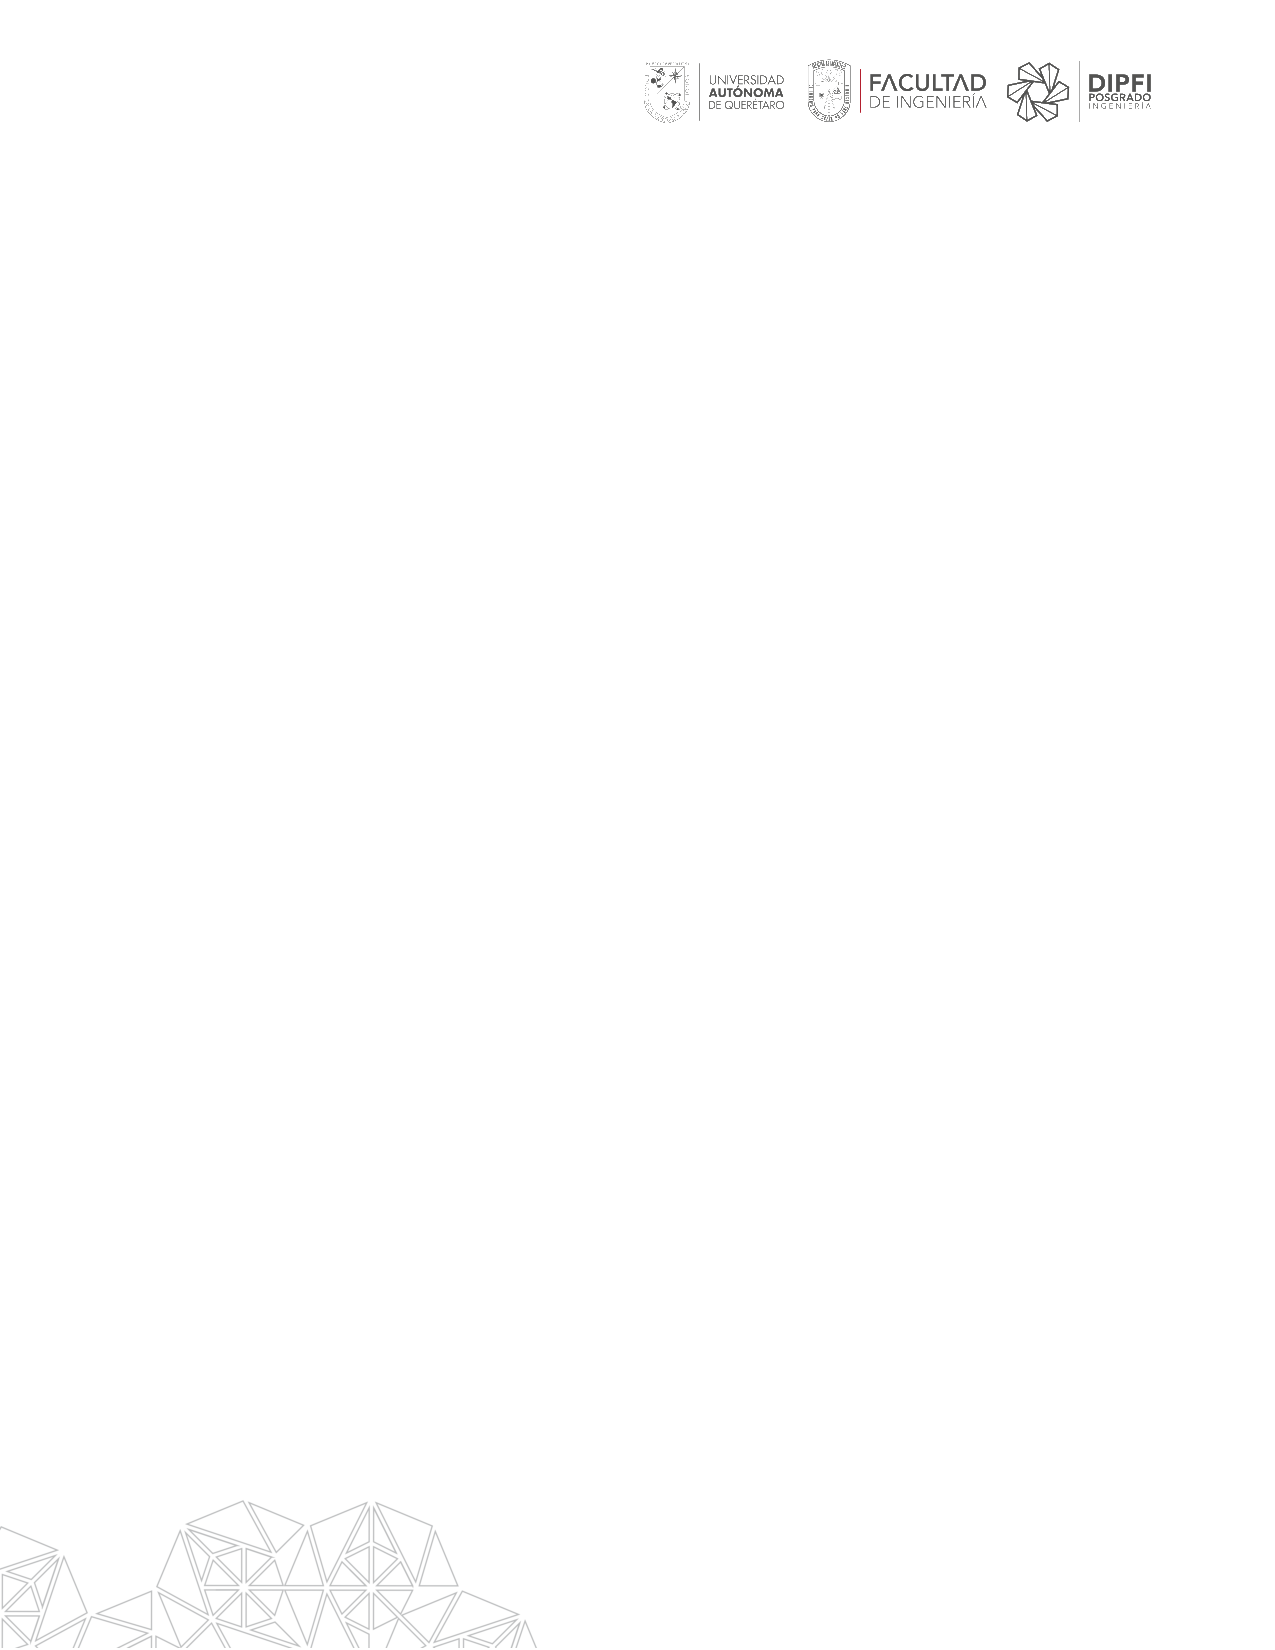
\includegraphics[width=\paperwidth]{BodyBackground.pdf}
	}
}


\pagenumbering{\Roman}
\setlength{\cftsecnumwidth}{3em} %Se cambia el espacio entre el item y el nombre de la seccion
\setlength{\cftsubsecindent}{1.3cm}
\setlength{\cftsubsubsecindent}{2.4cm}
\tableofcontents
\listoftables
\listoffigures




\pagestyle{plain}
\pagenumbering{arabic}




\section{Introducción/planteamiento del problema y justificación}
Tiene la intención de mostrar el problema que aborda la tesis, su justificación que consiste en la exposición de motivos o razones por las cuales se realizó la tesis, así como el contenido de los capítulos que la conforman. En este apartado es importante sustentar la relevancia social y/o científica del trabajo de tesis.

\section{Antecedentes}
Presentación de la revisión de estudios científicos relevantes tanto clásicos como actuales que tengan que ver con el problema específico que aborda la tesis. 

\section{Hipótesis}
En su caso.
Una hipótesis es una declaración que realizan los investigadores cuando especulan sobre el resultado de una investigación o experimento.
Son afirmaciones que pueden someterse a prueba y mostrarse como soluciones probablemente ciertas o no, sin que las creencias o los valores del investigador interfieran en el proceso de su comprobación.
Define la hipótesis como un enunciado que pone en relación dos o más variables que sirven de guía en el proceso de recogida de datos con el fin de comprobar y analizar lo que el investigador postula en ellas. La hipótesis debe formularse siempre en forma declarativa o expositiva.

\section{Objetivos}
Los objetivos expresan las situaciones que resolvieron/atendieron/explicaron. Deben de estar redactados en forma clara y concreta (redactados en infinitivo), y ser coherentes con la pregunta o preguntas de investigación, así como con el diseño metodológico.
Podrán dividirlos en objetivo general y objetivos específicos.

\section{Material y Métodos o Metodología}
Este apartado debe de ser descrito cuidadosamente de tal forma que quede claro qué es lo que se realizó.
Debe incluir:
\begin{itemize}
    \item Población. Si es el caso.
    \item Muestra y tipo de muestra (si es el caso).
    \item Descripción de las condiciones experimentales (si es el caso).
    \item Técnicas, instrumentos y procedimientos analíticos y estadísticos.
\end{itemize}

\section{Resultados y discusión}
Este es el apartado medular de la tesis pues es aquí donde se muestran los hallazgos. Los datos deben presentarse de manera organizada de tal forma que facilite la comprensión de los mismos. En el caso de que usen imágenes, figuras o tablas deben incluirse como parte del texto y no como un apartado por separado.
Deben de estar identificados con número y título.
La discusión consiste en la interpretación de los resultados comparándolos con los de otros autores o explicándolos a partir de la fundamentación teórica.

\section{Conclusiones}
Las conclusiones presentan el conocimiento generado en la tesis, deben de ser planteadas en forma explícita y clara.
Deberán ser congruentes con los objetivos y/o la o las preguntas de investigación.
Este apartado no es un resumen de resultados.



\nocite{*} % Para mostrar todas las refencias sin citarlas
\renewcommand{\refname}{Referencias bibliográficas}
\bibliographystyle{IEEEtran}
%\bibliographystyle{apalike}
\bibliography{referencias}

\end{document}
